\newpage
\section{System maintenance and RE}

Ever since software systems started becoming more and more complex, many of the larger systems that were based on monolithic architectures started migrating their systems to microservices-based architectures. Monzo, a UK-based digital bank, has implemented a system comprising approximately 2,800 microservices and counting~\citep{monzoMicroservices}. Because microservices and distributed systems are so complex, so is their maintenance. Moreover, there are other maintenance-related issues, like monitoring and collecting logs from independent microservices deployed in containers, and since microservices interact asynchronously, debugging failures is more complicated~\citep{Waseem_2021}. Maintenance of such systems requires thorough understanding, and since understanding such an extensive system is a complex process that cannot be accomplished in a single day, some other technique is needed to speed up the process. That is where reverse engineering plays a vital role. \textit{``The goal of reverse engineering is to reveal the logic, features, and functionalities embedded within the software''}\citep{digitalai_reverse_engineering}. Different techniques are employed to reverse engineer the system and reveal its logic and functionalities.

\subsection{RE Approaches}
\sloppy
There are three essential approaches for carrying out software reverse engineering. \textit{Observation-based analysis} which involves studying the exchange of information within the software to infer its functionality and behaviour. \textit{Disassembly} approach uses a disassembler to interpret and analyze the program's raw machine code. \textit{Decompilation} approach uses a decompiler to attempt a reconstruction of the program's source code in a high-level language, starting from machine code or bytecode~\citep{twoFacesOfSRE}.

\subsection{Reverse Engineering: Challenges and Insights}
Reverse engineering comes with several challenges. Rene R. Klosch discusses some of the challenges of reverse engineering~\citep{klosch1996reverse}. The paper includes that Legacy systems have source code that is poorly structured, which makes them challenging to analyze and understand. Large and complex systems require significant effort and expertise to be deconstructed. Moreover, maintenance engineers often lack sufficient knowledge about the original application domain, which is crucial for reverse engineering. The documentation, on the other hand, is often outdated or nonexistent, resulting in a lack of explicit information about the system's functionality and design.

\subsection{RE for Distributed Systems Maintenance}
Reverse engineering plays an essential role in maintaining and understanding large distributed systems. The approach used in the process depends on the requirement and overall specification of the project. In his thesis, Dan Calin Cosma discusses the role of reverse engineering in distributed systems maintenance\citep{CosmaReOODS}. Dan mentions that reverse engineering helps analyze the structure of distributed software systems, which often have complex dependencies due to their distributed nature. He also mentions that it can help identify functional units within the distributed systems. Furthermore, the thesis emphasizes that reverse engineering is not just about understanding the current system but also enabling its evolution by refactoring the current system without disrupting existing flows.

\begin{figure}[H]
    \centering
    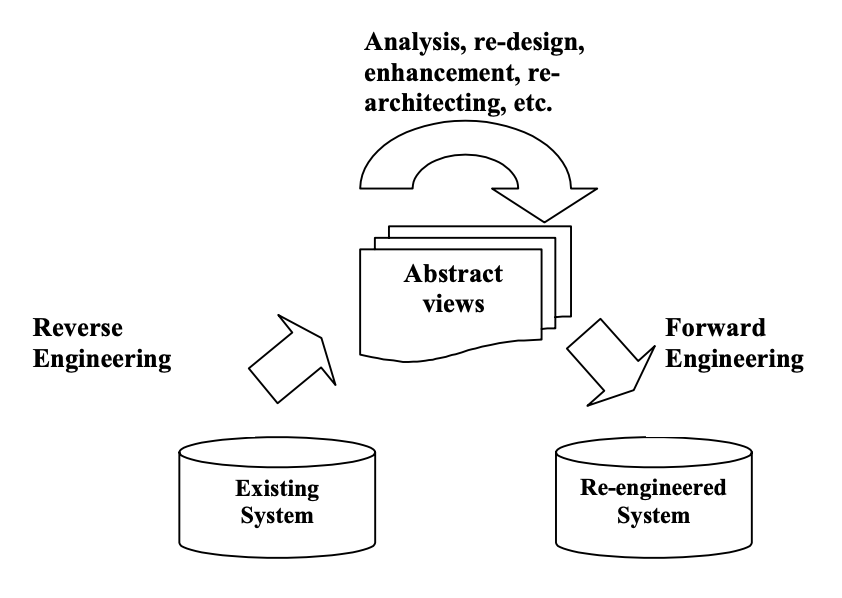
\includegraphics[width=0.7\textwidth]{figures/re_and_reengineering.png}
    \caption[Reverse engineering and re-engineering]{Reverse engineering and re-engineering (adapted from~\citep{SeMaintainance2001})}
    \label{fig:re_and_reengineering}
\end{figure}

In the later chapters of this report, we will discuss a framework that uses static analysis of source code. This framework aids reverse engineering by disassembling the system and generating valuable insights.